\documentclass[11pt,a4paper]{article}
\synctex=1
\usepackage[utf8]{inputenc}
\usepackage[margin=1cm, bottom=2cm]{geometry}
\usepackage{graphicx}
\usepackage{amsmath}
\usepackage{amssymb}
\usepackage{listings}
\usepackage{textcomp}
\usepackage{courier}
\usepackage[hangul]{kotex}


\linespread{1.3}

\begin{document}
\begin{center}
\vspace*{2cm}
{\fontsize{50}{50} 자료구조와 실습
\vspace{1cm}
\\연습문제}
\vspace{9cm}	

\LARGE
\begin{tabular}{rl}
학번 : & 2016110056\\ 
학과 : & 불교학부 \\
이름 : & 박승원\\
날짜 : & \today
\end{tabular}
\vspace{1cm}


\includegraphics[width=0.5\textwidth]{logo.jpg}

\end{center}
\newpage


\noindent
\begin{enumerate}
	

\item 리스트에 대한 설명 중 틀린 것은?
\begin{enumerate}
	\item 구조체도 리스트의 요소가 될 수 있다.
	\item 리스트의 요소간에는 순서가 있다.
	\item 리스트는 여러 가지 방법으로 구현될 수 있다.
	\item \fbox{리스트는 집합과 동일하다.}
\end{enumerate}

\item 다음은 순차적 표현과 연결된 표현을 비교한 것이다. 설명이 틀린 것을 모두 표시하시오.
	\begin{enumerate}
	\item \fbox{연결된 표현은 포인터를 가지고 있어 상대적으로 크기가 작아진다.}
	\item 연결된 표현은 삽입이 용이하다.
	\item \fbox{순차적 표현은 연결된 표현보다 접근 시간이 많이 걸린다.}
	\item 연결된 표현으로 작성된 리스트를 2개로 분리하기가 쉽다.
	\end{enumerate}
	
\item 다은은 연결 리스트에서 있을 수 있는 여러 가지 경우를 설명한다. 잘못된 항목은?
	\begin{enumerate}
		\item 정적인 데이터보다는 변화가 심한 데이터에서 효과적인 방법이다.
		\item 모든 노드는 데이터와 링크(포인터)를 가지고 있어야 한다.
		\item \fbox{연결 리스트에서 사용한 기억 장소는 다시 사용할 수 있다.}
		\item 데이터들이 메모리상에 흩어져서 존재할 수 있다.
	\end{enumerate}

\item 삽입과 삭제 작업이 자주 발생할 때 실행 시간이 가장 많이 소요되는 자료구조는?
	\begin{enumerate}
		\item \fbox{배열로 구현된 리스트}
		\item 단순 연결 리스트
		\item 원형 연결 리스트
		\item 이중 연결 리스트
	\end{enumerate}

\item 다음 중 NULL 포인터(Null pointer)가 존재하지 않는 구조는 어느 것인가?
	\begin{enumerate}
		\item 단순 연결 리스트
		\item 원형 연결 리스트
		\item \fbox{이중 연결 리스트}
		\item 헤더 노드를 가지는 단순 연결 리스트
	\end{enumerate}

\item 원형 연결 리스트에 대한 설명 중 틀린 것은?
	\begin{enumerate}
		\item 모든 노드들이 연결되어 있다.
		\item 마지막에 삽입하기가 간단하다.
		\item 헤더 노드를 가질 수 있다.
		\item \fbox{최종 노드 포인터가 NULL이다.}
	\end{enumerate}

\item 리스트의 n번째 요소를 가장 빠르게 찾을 수 있는 구현 방법은 무엇인가?
	\begin{enumerate}
		\item \fbox{배열}
		\item 단순 연결 리스트
		\item 원형 연결 리스트
		\item 이중 연결 리스트
	\end{enumerate}
	
\item 단순 연결 리스트의 노드 포인터 p가 마지막 노드를 가리킨다고 할 때, 다음 수식 중 참인 것은?
	\begin{enumerate}
		\item last == NULL
		\item $last\rightarrow data == NULL$
		\item \fbox{$last\rightarrow link == NULL$}
		\item $last\rightarrow link\rightarrow link == NULL$
	\end{enumerate}

\item 단순 연결 리스트의 노드들을 노드 포인터 p로 탐색하고자 한다. p가 현재 가리키는 노드에서 다음 노드로 가려면 어떻게 하여야 하는가?
	\begin{enumerate}
		\item p++;
		\item p$--$;
		\item \fbox{p=p$\rightarrow$ link;}
		\item p=p$\rightarrow $data;
	\end{enumerate}
	
\item 단순 연결 리스트의 관련 함수 f가 헤드 포인터 head를 변경시켜야 한다면 함수 매개 변수로 무엇을 받아야 하는가?
	\begin{enumerate}
		\item head
		\item \fbox{\&head}
		\item *head
		\item head$\rightarrow$link;
	\end{enumerate}
\lstset{language=C, tabsize=4, frame=single, showstringspaces=false, breaklines=true, columns=flexible, basicstyle=\ttfamily\small}


\item A라는 공백 상태의 리스트가 있다고 가정하자. 이 리스트에 대하여 다음과 같은 연산들이 적용된 후의 리스트의 내용을 그려라.
\begin{lstlisting}[frame=none]
add_first(A, "first");
add(A, 1, "second");
add_last(A,"third");
add(A,2,"fourth");
add(A,4,"fifth");
delete(A,2);
delete(A,2);
replace(A, 1, "sixth");
\end{lstlisting}
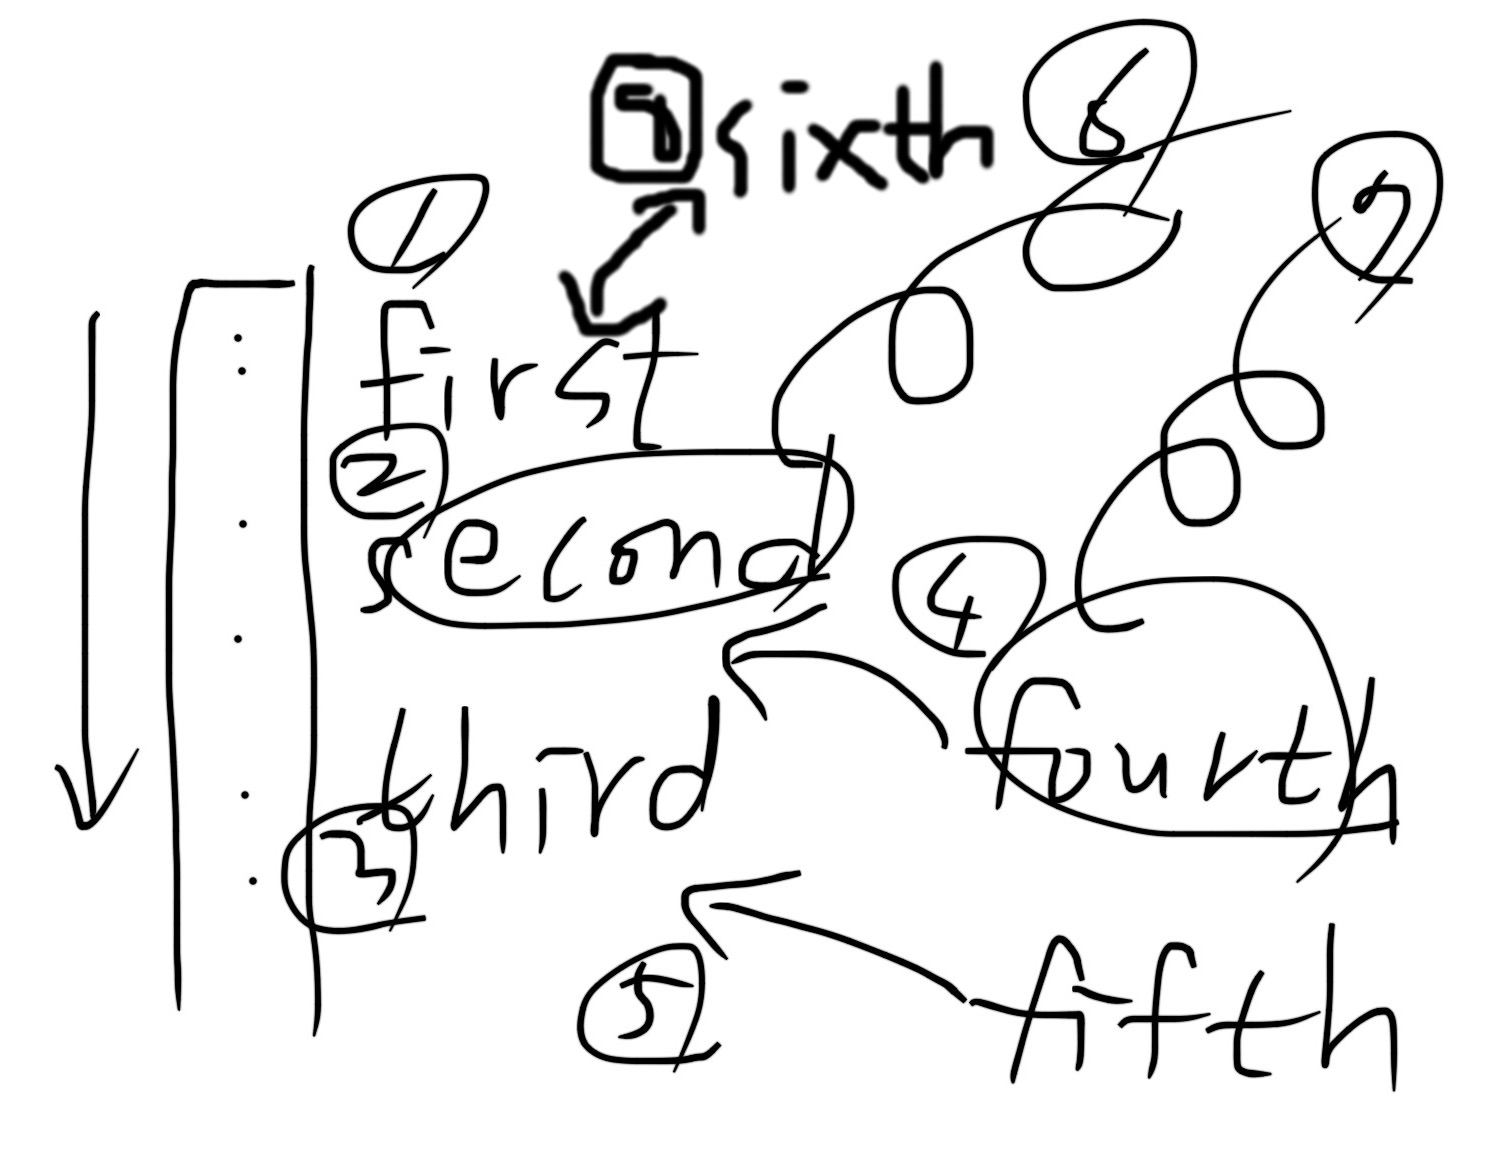
\includegraphics[width=\textwidth]{11.jpg}


\item 배열을 이용하여 구현한 리스트의 경우, 리스트의 연산 중 일부 연산만 구현되어 있다. 본문의 코드를 참조하여 리스트 ADT의 나머지 연산들도 구현하여 보라.

\item 단순 연결 리스트에서 삭제 함수 delete 함수는 실제로는 헤드 포인터와 선행 노드 포인터의 2개의 매개변수만 있으면 작성이 가능하다. 이들 두 매개 변수만을 사용하여 다시 작성하라.
\lstinputlisting[language=C, frame=single, title=앞으로 계속 사용하게 될 헤더화일 list.h]{list.h}

\item 단순연결 리스트에 정수가 저장되어 있다. 단순 연결 리스트의 모든 데이터 값을 더한 합을 출력하는 프로그램을 작성하시오.

\item 단순 연결 리스트에서 특정한 데이터 값을 갖는 노드의 개수를 계산하는 함수를 작성하여라.

\item 단순 연결 리스트에서 탐색 함수를 참고하여 특정한 데이터값을 갖는 노드를 삭제하는 함수를 작성하라.

\item 단순 연결 리스트의 헤드 포인터가 주어져 있을 때, 첫 번째 노드에서부터 하나씩 건너서 있는 노드를 삭제하는 함수를 작성하라. 즉, 홀수번째 있는 노드들이 전부 삭제된다.
\lstinputlisting[language=C,frame=single,title=13-17]{list.c}
\includegraphics[width=\textwidth]{list.png}

\item 두개의 단순 연결 리스트 A,B가 주어져 있을 경우, alternate 함수를 작성하라. alternate 함수는 A와 B로부터 노드를 번갈아 가져와서 새로운 리스트 C를 만드는 연산이다. 만약 입력 리스트 중에서 하나가 끝나게 되면 나머지 노드들을 전부 C로 옮긴다. 함수를 구현하여 올바르게 동작하는지 테스트하라. 작성된 함수의 시간 복잡도를 구하라.
\lstinputlisting[language=C, frame=single]{18.c}
\includegraphics[width=\textwidth]{18.png}

\item 보통 연결 리스트에서는 선행 노드를 알아야만이 노드를 삭제할 수 있다. 그러나, 다음과 같이 하면 선행 노드를 모르고도 노드를 삭제할 수 있다. 먼저 원형 연결 리스트라고 가정하자. 어떤 노드를 가리키는 포인터 x가 주어진 경우, 그 노드의 후속 노드를 쉽게 찾을 수 있다. 후속 노드를 y라고 한다면 x에 y의 데이터 필드값을 복사한다. 그리고 y를 삭제한다. 그러면 실질적으로는 x가 삭제된 것처럼 된다. 이런 식으로 노드를 삭제하는 함수 remove_node2를 작성하고 구현하여 테스트하라.
\lstinputlisting[language=C,frame=single]{21.c}
\includegraphics[width=\textwidth]{21.png}

\item 단순 연결 리스트 C를 두개의 단순 연결 리스트 A와 B로 분리하는 함수 split를 작성하여 보자. C의 홀수번째 노드들은 모두 A로 이동되고 C의 짝수번째 노드들은 모두 B로 이동된다. 이 함수가 C를 변경하여서는 안된다. 작성된 알고리즘의 시간 복잡도를 구하고 구현하여 수행하여 보자.
\lstinputlisting[language=C, frame=single]{20.c}
\includegraphics[width=\textwidth]{20.png}
\item 이항계수(binomial coefficient)를 계산하는 순환 함수를 작성하라. 이항계수는 다음과 같이 순환적으로 정의된다. 반복 함수로도 구현해보라.\\

\begin{lstlisting}
int nCr(int n, int r)
{
	if(r==0 || r==n) return 1;
	return nCr(n-1, r-1) + nCr(n-1, r);
}

//반복함수
int factorial(int n) {
	int r = 1;
	for(int i=1; i<=n; i++) r *= i;
	return r;
}
int nPr(int n, int r) {
	return factorial(n)/factorial(r);
}
int nCr(int n, int r)
{
	return nPr(n, r)/factorial(r);
}
\end{lstlisting}
\item 
\begin{lstlisting}
struct SparseMatrix {//첫번째 노드에서는 행렬의 너비 높이 0이 아닌 값의 갯수이고, 
	int x, y, v;//두번째 노드부터는 x,y좌표와 그 값이다.
	struct SparseMatrix* node;
} SparseMatrix;
\end{lstlisting}
\item Ackermann 함수는 다음과 같이 순환적으로 정의된다.

A(0, n) = n+1\\
A(m, 0) = A(m-1, 1)\\
$ A(m, n) = A(m-1, A(m, n-1)) m,n\geqq 1 $

\begin{enumerate}
	\item A(3,2)와 A(2,3)의 값을 구하시오. 29, 9
	\item Ackermann 함수를 구하는 순환적인 프로그램을 작성하시오.
	\begin{lstlisting}
	int A(int m, int n) {
		if(m == 0) return n+1;
		if(n == 0) return A(m-1, 1);
		return A(m-1, A(m, n-1));
	}
	\end{lstlisting}
	
	\item 위의 순환적인 프로그램을 for, while, do와 같은 반복구조를 사용한 비순환적 프로그램으로 바꾸시오.
	\begin{lstlisting}
	int Stack[MAX];
	int top = -1;
	int Push(int value);
	int Pop();
	int Ackermann(int m, int n);
	int main()
	{
		int m, n;
		printf("Enter two values : ");
		scanf("%d %d", &m, &n);
		printf("The result is %d.\n", Ackermann(m, n));
		return 0;
	}
	
	int Push(int value)
	{
		if ( top >= MAX - 1 ) {
			printf("Stack overflow\n");
			return -1;
		}
		Stack[++top] = value;
		return value;
	}
	
	int Pop()
	{
		if ( top < 0 ) {
			return -1;
		}
		return Stack[top--];
	}
	
	int Ackermann(int m, int n)
	{
		while ( 1 ) {
			if ( 0 == m ) {
				++n;
				m = Pop();
				if ( m == -1 ) return n;
			} else if ( 0 == n ) {
				--m;
				++n;
			} else {
				if ( Push(m-1) == -1 )	exit(1);
				--n;
			}
		}
		return -1;
	}
	
	\end{lstlisting}
\end{enumerate}
	
\item 본문의 순환적인 피보나치 수열 프로그램과 반복적인 피보나치 수열 프로그램의 수행 시간을 측정하여 비교하라. 어떤 결론을 내릴 수 있는가? 

반복적인 프로그램이 더 빠르다. 재귀적인 프로그램에서는 메모리의 할당, 함수의 호출 등의 작업이 일어나기 때문으로 보인다.

\item 순환 호출에서는 순환 호출을 할때마다 문제의 크기가 작아져야 한다.
\begin{enumerate}
	\item 팩토리얼 계산 문제에서 순환 호출이 일어날 때마다 문제가 어떻게 작아지는가?
	
	계산하고자 하는 입력값이 1씩 작아진다.
	\item 하노이의 탑에서 순환 호출이 일어날 때마다 문제가 어떻게 작아지는가?
	
	옮기는 더미가 하나씩 줄어든다.
\end{enumerate}


\end{enumerate}
\lstinputlisting[language=C++,frame=single, title=Hanoi tower]{hanoi.cc}

\vspace{2cm}
{\Huge 소감}

순환구조를 반복구조로 바꾸는 것이 함수만 주고 구하라니 굉장히 어려웠다. 수열의 진행을 하나하나 조사해야 되었다. 만약 재귀함수가 없었다면 얼마나 불편했을까하고 생각해보게 되었다. 에커만 함수는 결국 인터넷을 참조하는 수밖에 없었다. 그런데, 이상한 것이 인터넷의 프로그램도 스택을 이용하여 계산을 하는 것이라, 반복문이라고 보기에는 이상했다. 더 이상 에커만 함수를 연구하는 것이 생산적이지는 않을 것 같아 더 연구하지는 않았다. 대신 하노이 탑 재귀적으로 프로그래밍하는 것을 해보았다. 프로그래머의 입장에서 프로그래밍에서 가장 중요한 것은 반복되는 가장 작은 단위를 찾는 것인데, 재귀함수는 이런 점에 가장 부합한다. 재귀함수를 잘 활용하는 것이 매우 중요하다고 생각한다.

그리고, 이책에서는 recursive를 순환적인 프로그램으로 해석했다. 다른 책에서는 대부분 재귀적인 프로그램으로 해석하는데, 여기서는 용어가 달라 헷갈린다. 순환과 반복이란 용어가 거의 비슷한 뜻이니 재귀라는 단어를 쓰면 좋겠다.
\newpage
\includegraphics[height=\textheight]{23.png}
\end{document}
